% !TEX root = CartaPerali_Report.tex

\section{Results}
\label{sec:results}
\noindent In this section the test results are presented. The confusion matrix in Fig. \ref{fig:conf_matrix_cnn} shows the affective ability of the model in making predictions. In Table \ref{table:Preprocessing} some results of the proposed model with different learning rates and number of epochs are shown. It can be observed how {\it{Configuration A}} yields the best performance in test phase, achieved in this work.

\begin{figure}[h]
			\centering
	    	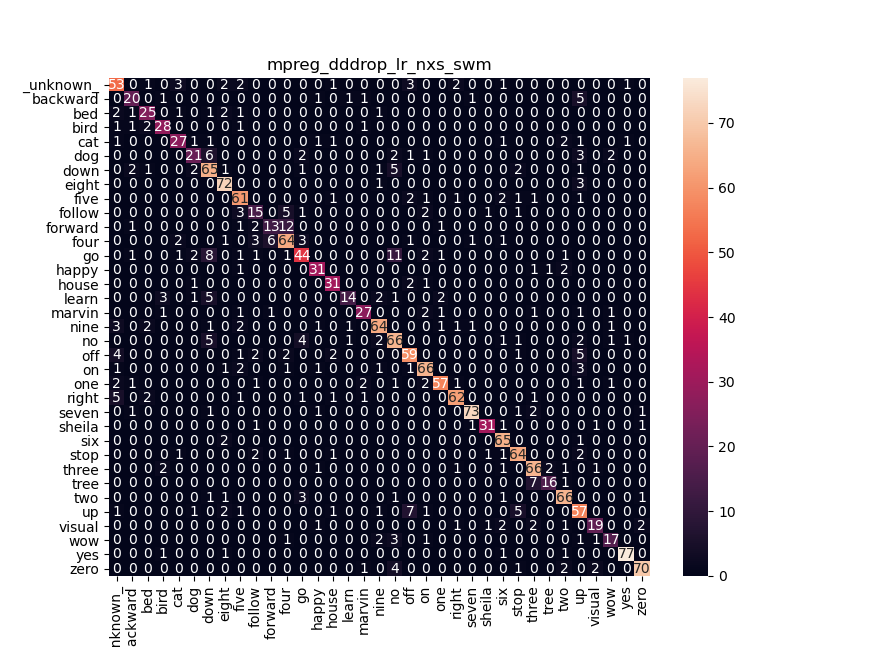
\includegraphics[width=10cm, height=8cm]{conf_matrix_cnn_dii_cm}
	    	\caption{Confusion matrix}
	    	\label{fig:conf_matrix_cnn}
\end{figure} 

\begin{table*}[ht]
	\centering
	\begin{tabular}{|c c c c c c c c|}
		\hline
		Configuration & Preprocess & Optimizer & LR & Trainable param. & Epochs  & Labels & Accuracy \\
		\hline
		A & Specgram & Adam & 5e-4 & 1,459,155 & 10 & 35 & 80.3\% \\
		B & Specgram & Adam & 1e-4 & 1,459,155 & 20 & 35 & 79.2\% \\
		C & Specgram & Adam & 5e-5 & 1,459,155 & 25 & 35 & 78.9\% \\
		\hline
	\end{tabular}
	\caption{Preprocessing}
	\label{table:Preprocessing}
\end{table*}